% !TEX program = pdflatex
\documentclass[12pt,a4paper]{ctexart}

% ========== 页面设置 ==========
\usepackage[top=2.5cm, bottom=2.5cm, left=3.0cm, right=2.5cm]{geometry}
\usepackage{setspace}
\onehalfspacing
\parindent=2em

% ========== 字体 ==========
\usepackage{times}

% ========== 图表支持 ==========
\usepackage{graphicx}
\usepackage{caption}
\usepackage{float}

% ========== 超链接 ==========
\usepackage[colorlinks=true, linkcolor=black, citecolor=black, urlcolor=black]{hyperref}

% ========== 页眉页脚 ==========
\usepackage{fancyhdr}
\pagestyle{fancy}
\fancyhf{}
\fancyhead[L]{\zihao{6}\rmfamily 江苏大学课程论文}
\fancyhead[R]{\zihao{6}\rmfamily 太阳能光伏发电技术综述}
\fancyfoot[C]{\zihao{6}\thepage}
\renewcommand{\headrulewidth}{0.4pt}
\renewcommand{\footrulewidth}{0pt}
\fancypagestyle{plain}{
    \fancyhf{}
    \fancyfoot[C]{\zihao{6}\thepage}
    \renewcommand{\headrulewidth}{0pt}
}
\setlength{\headheight}{14.5pt}
\addtolength{\topmargin}{-2.5pt}

% ========== 标题格式 ==========
\ctexset{
    section/format = \heiti\zihao{3},
    subsection/format = \songti\bfseries\zihao{4},
}

\begin{document}

% ==================== 封面 ====================
\thispagestyle{empty}
\begin{center}
    \vspace*{2cm}
    
    {\heiti\zihao{3} 太阳能光伏发电技术综述}
    
    \vspace{3cm}
    
    {\songti\zihao{4}
    专业班级：微电子2201\hspace{3em}学生姓名：超级老付
    
    \vspace{0.5cm}
    
    指导教师：李四\hspace{4.5em}职\quad 称：讲师
    }
\end{center}

\vspace{1cm}

% ==================== 中文摘要 ====================
\begin{center}
    {\heiti\zihao{4} 摘\quad 要}
\end{center}

太阳能光伏发电是可再生能源利用的重要方向，对推动能源结构转型和实现碳中和目标具有重要意义。本文系统综述了晶硅电池、薄膜电池和钙钛矿电池三类光伏技术的发展现状与技术特征，分析了光伏发电在集中式电站和分布式应用场景中的部署进展，展望了钙钛矿叠层电池等前沿技术的未来发展方向。

\vspace{12bp}
\noindent{\heiti\zihao{4} 关键词：} 光伏发电；新能源；钙钛矿电池；碳中和

% ==================== 目录 ====================
\newpage
\tableofcontents

% ==================== 正文 ====================
\newpage

\section{引言}

随着全球气候变化问题日益严峻，推动能源结构向清洁低碳方向转型已成为国际社会的普遍共识。太阳能光伏发电因其资源丰富、技术成熟、成本快速下降等优势，在全球能源转型中扮演着关键角色。据国际能源署（IEA）数据，2024年全球光伏累计装机容量已超过1.5~TW，年新增装机超过400~GW\cite{ref1}。

近年来，光伏电池技术取得了显著进展。晶硅电池效率持续提升，钙钛矿太阳能电池更是以惊人的速度发展，其实验室效率已从2009年的3.8\%提升至2024年的26\%以上\cite{ref2}。图\ref{fig:eff}展示了不同类型光伏电池的效率发展趋势。

\section{光伏电池技术分析}

\subsection{晶硅电池技术}

晶硅电池是目前市场占有率最高的光伏技术，约占全球光伏市场的95\%。其中，钝化发射极和背面电池（PERC）技术已实现大规模量产，异质结（HJT）和隧穿氧化层钝化接触（TOPCon）技术代表了新一代高效晶硅电池的发展方向。

\subsection{薄膜电池技术}

薄膜电池主要包括碲化镉（CdTe）、铜铟镓硒（CIGS）和非晶硅（a-Si）等类型。薄膜电池具有弱光性能好、温度系数低、适合建筑一体化等优势，但其市场份额相对较小。

\subsection{钙钛矿电池技术}

钙钛矿太阳能电池是近年来发展最为迅速的新型光伏技术。其材料成本低廉、制备工艺简单，且可与晶硅电池组成叠层结构，理论效率可超过40\%。然而，钙钛矿电池的长期稳定性和大面积制备仍是亟待突破的关键问题。

\begin{center}
    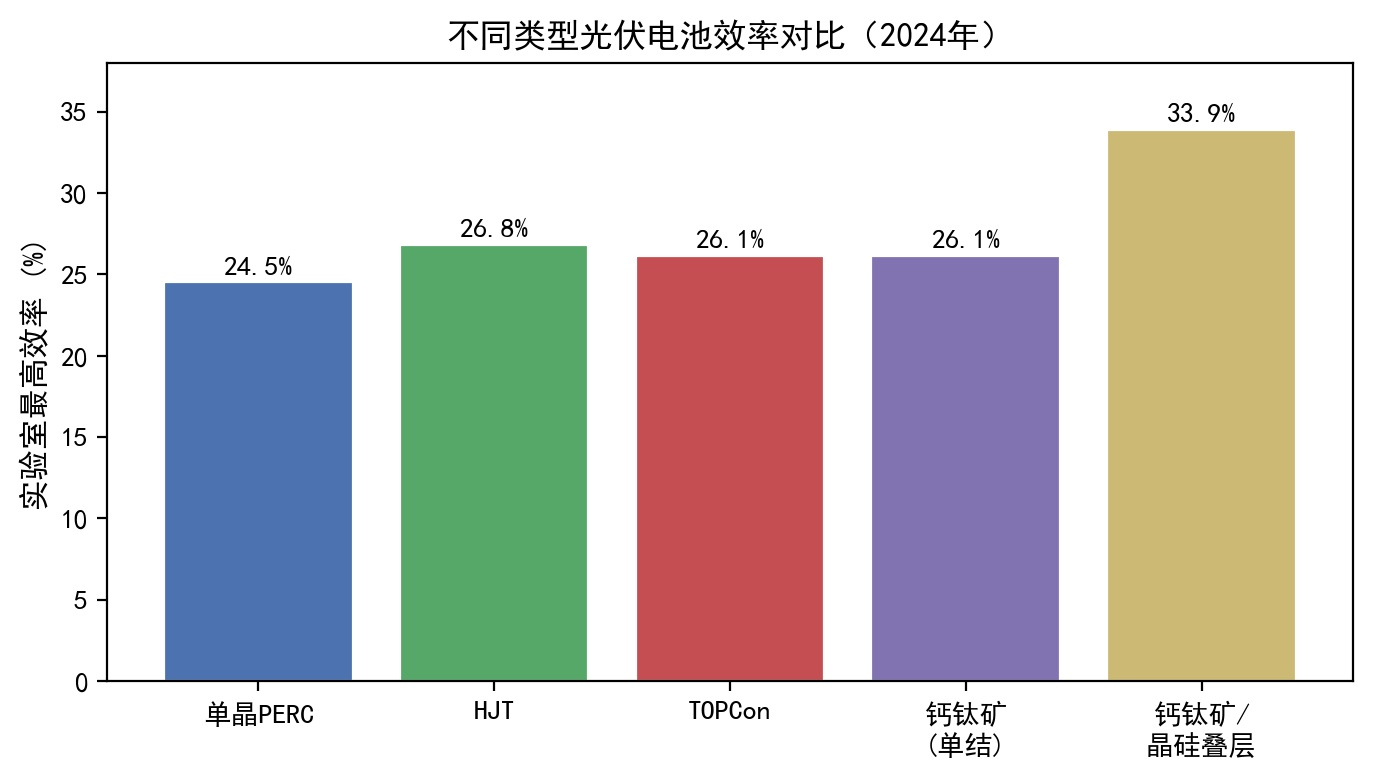
\includegraphics[width=0.7\textwidth]{figures/demo_chart.jpg}
    \captionof{figure}{不同类型光伏电池效率对比（2024年）}\label{fig:eff}
\end{center}

\section{应用现状与发展趋势}

光伏发电的应用场景不断拓展，从大规模荒漠电站到屋顶分布式光伏，从农光互补到水面漂浮式光伏，多元化应用格局已经形成。在全球碳中和目标的驱动下，光伏发电预计将在2050年占全球发电量的30\%--40\%。

\section{结论}

\subsection{主要结论}

本文系统综述了太阳能光伏发电技术的发展现状和应用前景，主要得出以下结论：（1）晶硅电池仍将在一段时间内保持市场主导地位，但效率提升空间有限；（2）钙钛矿太阳能电池具有广阔的发展前景，有望成为下一代主流光伏技术；（3）光伏发电成本的持续下降将加速其在全球能源结构中的渗透。

\subsection{研究展望}

未来研究应重点关注钙钛矿电池的稳定性提升技术、大面积制备工艺以及叠层电池的产业化路径。

% ==================== 参考文献 ====================
\addcontentsline{toc}{section}{参考文献}
\renewcommand{\refname}{}
\begin{center}
    {\zihao{-2}\bfseries 参考文献}
\end{center}
\vspace{12bp}
\begin{thebibliography}{99}
\bibitem{ref1} International Energy Agency. World Energy Outlook 2024[R]. Paris: IEA, 2024.
\bibitem{ref2} 李五, 赵六. 钙钛矿太阳能电池效率提升策略研究[J]. 太阳能学报, 2024, 45(3): 1-12.
\end{thebibliography}

\end{document}
